\documentclass[a4paper, 12pt]{article}
\usepackage{amsmath}
\usepackage{amsthm}
\usepackage{amssymb}
\usepackage{longtable}
\usepackage{pdflscape}
\usepackage{algorithm}
\usepackage{graphicx}
\usepackage[noend]{algpseudocode}
\usepackage{url}
\usepackage{tikz}
\usetikzlibrary{arrows}

\newlength\tindent
\setlength{\tindent}{\parindent}
\setlength{\parindent}{0pt}
\renewcommand{\indent}{\hspace*{\tindent}}

\newtheorem{thm}{Theorem}
\newtheorem{cor}{Corollary}[thm]
\newtheorem{lemma}{Lemma}[thm]

\title{COMP 307 Assignment 3}
\author{Daniel Braithwaite}

\begin{document}
	\pagenumbering{gobble}
	\maketitle
	\newpage
  	\pagenumbering{arabic}
  	
	\section{Naive Bayes Method}
		\subsection{Part 1}
			\begin{center}
\begin{tabular}{|c|c|c|}
\hline
Feature & Spam & Non Spam\\\hline$F_0$ & 0.6730769230769231 & 0.36\\
$F_1$ & 0.5961538461538461 & 0.58\\
$F_2$ & 0.46153846153846156 & 0.3466666666666667\\
$F_3$ & 0.6153846153846154 & 0.4\\
$F_4$ & 0.5 & 0.34\\
$F_5$ & 0.36538461538461536 & 0.47333333333333333\\
$F_6$ & 0.7884615384615384 & 0.5066666666666667\\
$F_7$ & 0.7692307692307693 & 0.35333333333333333\\
$F_8$ & 0.34615384615384615 & 0.24666666666666667\\
$F_9$ & 0.6730769230769231 & 0.29333333333333333\\
$F_{10}$ & 0.6730769230769231 & 0.5866666666666667\\
$F_{11}$ & 0.7884615384615384 & 0.34\\
\hline
\end{tabular}
			\end{center}
			
		\subsection{Part 2}
			\begin{center}
				\begin{tabular}{|c|c|c|}
				\hline
Class & Spam Prob & Non Spam Prob\\
\hline
Not Spam & 0.000005 & 0.000495\\
Spam & 0.000072 & 0.000045\\
Spam & 0.000234 & 0.000140\\
Not Spam & 0.000008 & 0.000647\\
Not Spam & 0.000077 & 0.000100\\
Spam & 0.000074 & 0.000050\\
Not Spam & 0.000005 & 0.000354\\
Not Spam & 0.000081 & 0.000424\\
Spam & 0.000234 & 0.000041\\
Not Spam & 0.000028 & 0.000734\\
\hline
\end{tabular}
			\end{center}
			
		\subsection{Part 3}
			Say we where given a feature vector and we knew the following things. It contained the word "Viagra" and contained a significant amount of CAPS. Knowing this we would make the probability of finding the words "MILLION DOLLARS" in the email higher than if we knew nothing.
			\\\\
			For a given email the presence of a feature means the email is more likely to be spam. So if features are not independent this means that the presence of one feature means other features are more likely to be present. Skewing the classifier in favor of the Spam class.			
	
	\section{Reasoning Under Uncertainty Basics}
		\subsection{Part 1}
			To fill out the probability table we need to solve the following formula
			\begin{align*}
				P(X = x, Y = y)
			\end{align*}
			Which by using the \textbf{chain rule} we get this to be 
			\begin{align*}
				P(X = x, Y = y) = P(X = x) * P(Y = y|X = x)
			\end{align*}
				
			So we compute the table with the following computation				
				
			\begin{align*}
				P(X = 0, Y = 0) = P(X = 0) * P(Y = 0|X = 0) = 0.3 * 0.3 = \frac{9}{100}\\
				P(X = 0, Y = 1) = P(X = 0) * P(Y = 1|X = 0) = 0.3 * 0.7 = \frac{21}{100}\\
				P(X = 1, Y = 0) = P(X = 1) * P(Y = 0|X = 1) = 0.7 * 0.8 = \frac{14}{100}\\
				P(X = 1, Y = 1) = P(X = 1) * P(Y = 1|X = 1) = 0.7 * 0.2 = \frac{7}{100}
			\end{align*}
			
			\begin{center}
				\begin{tabular}{|c|c|c|}
					\hline
					X & Y & P(X,Y)\\
					\hline
					0 & 0 & $\frac{9}{100}$\\
					0 & 1 & $\frac{21}{100}$\\
					1 & 0 & $\frac{14}{25}$\\
					1 & 1 & $\frac{7}{50}$\\
					\hline
				\end{tabular}
			\end{center}
			
		\subsection{Part 2}
			To compute the full joint probability table we need to simply $P(X=x,Y=y,Z=z)$ by first applying the chain rule and then applying the fact that $Z$ is independent to $X|Y$
			
			\begin{align*}
				P(X=x,Y=y,Z=z) = P(X=x) * P(Y=y|X=x) * (Z=z|X=x,Y=y)\\
				= P(X=x) * P(Y=y|X=x) * P(Z=z|Y=y)
			\end{align*}
			
			Using this formula we can compute the missing entries in the table			

			\begin{equation*}
				\begin{split}
					P(X=0,Y=0,Z=0) & = P(X=0) * P(Y=0|X=0) * P(Z=0|Y=0) 
					\\					
					& = 0.3 * 0.3 * 0.6 = 0.054
				\end{split}
			\end{equation*}								
					
			\begin{equation*}
				\begin{split}
					P(X=1,Y=0,Z=1) & = P(X=1) * P(Y=0|X=1) * P(Z=1|Y=0)
					\\ 
					& = 0.7 * 0.8 * 0.4 = 0.224
				\end{split}
			\end{equation*}
			
			\begin{equation*}
				\begin{split}
					P(X=1,Y=1,Z=0) & = P(X=1) * P(Y=1|X=1) * P(Z=0|Y=1)
					\\ 
					& = 0.7 * 0.2 * 0.8 = 0.112
				\end{split}
			\end{equation*}
			
			\begin{equation*}
				\begin{split}
					P(X=1,Y=1,Z=1) & = P(X=1) * P(Y=1|X=1) * P(Z=1|Y=1)
					\\
					& = 0.7 * 0.2 * 0.2 = 0.028
				\end{split}
			\end{equation*}						
	
			From this we get the full table to be 	
	
			\begin{center}
				\begin{tabular}{|c|c|c|c|}
					\hline
					X & Y & Z & P(X,Y,Z)\\
					\hline
					0 & 0 & 0 & \textbf{0.054}\\
					0 & 0 & 1 & 0.036\\
					0 & 1 & 0 & 0.168\\
					0 & 1 & 1 & 0.042\\
					1 & 0 & 0 & 0.336\\
					1 & 0 & 1 & \textbf{0.224}\\
					1 & 1 & 0 & \textbf{0.112}\\
					1 & 1 & 1 & \textbf{0.028}\\
					\hline
				\end{tabular}
			\end{center}				
	
		\subsection{Part 3}
			\subsubsection{Section I}
				\begin{equation}
					\begin{split}
						P(Z=0) & = P(X=0,Y=0,Z=0)
						\\
						& + P(X=0,Y=1,Z=0)
						\\
						& + P(X=1,Y=0,Z=0)
						\\
						& + P(X=1,Y=1,Z=0)	
						\\\\
						& = 0.054 + 0.168 + 0.336 + 0.112
						\\
						& = 0.67
					\end{split}
				\end{equation}								
				\subsubsection{Section II}
				If X and Z are independent then we will have that $P(X|Z) = P(X)$. So we check the following
				
				\begin{align*}
					P(X=0|Z=0) = \frac{P(X=0,Z=0)}{P(Z=0)}
				\end{align*}
				
				We know what $P(Z=0)$ is but we need to find $P(X=0,Z=0)$ which we can do by using the joint distribution from Question 2
				
				\begin{equation}
					\begin{split}
						P(X=0,Z=0) & = P(X=0,Y=0,Z=0)
						\\
						& + P(X=0,Y=1,Z=0)
						\\
						& = 0.54 + 0.168
						\\
						& = 0.222
					\end{split}
				\end{equation}
				
				We can now solve for $P(X=0|Z=0)$.
				\begin{align*}
					P(X=0|Z=0) = \frac{0.222}{0.67} = 0.331
				\end{align*}
				
				And $P(X=0|Z=0) = 0.331 \neq 0.3 = P(X=0)$. So X and Z are dependent.
				
		\subsection{Part 4}
			Both these can be computed from the joint probability table		
		
			\subsubsection{Section I}
				\begin{align*}
					P(X=1,Y=0|Z=1) = P(X=1,Y=0,Z=1) = 0.224
				\end{align*}
			
			\subsubsection{Section II}
				\begin{align*}
					P(X=0|Y=0,Z=0) = P(X=0,Y=0,Z=0) = 0.054
				\end{align*}
	\section{Bayesian Networks}
		\subsection{Part 1}
			\subsubsection{Variables}
				\begin{enumerate}
					\item Working Location (W) has options (u, h)
					\item Logged In (I) has options (true, false)
					\item Light On (O) has options (true, false)
					\item Lectures (L) has options (true, false)
					\item Meetings (M) has options (true, false)
				\end{enumerate}
				
			\subsubsection{Network Graph}
				The Bayesian network i designed for this problem has the following structure 
				\begin{figure}[H]
\centering
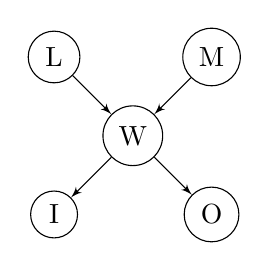
\begin{tikzpicture}
\tikzset{vertex/.style = {shape=circle,draw,minimum size=1.5em}}
\tikzset{edge/.style = {->,> = latex'}}
% vertices
\node[vertex] (l) at  (-1, 1)  {L};
\node[vertex] (m) at  (1, 1)   {M};
\node[vertex] (w) at  (0, 0)   {W};
\node[vertex] (i) at  (-1, -1) {I};
\node[vertex] (o) at  (1, -1)  {O};
%edges
\draw[edge] (l) to (w);
\draw[edge] (m) to (w);
\draw[edge] (w) to (i);
\draw[edge] (w) to (o);
\end{tikzpicture}
\end{figure}
			
			\subsubsection{Prior Probability}
			
				The prior probability table for L is\\
				\begin{tabular}{|c|c|}
					\hline
					L & P(L)\\
					\hline
					0 & 0.4\\
					1 & 0.6\\
					\hline
				\end{tabular}
				\\\\
				The prior probability table for M is\\
				\begin{tabular}{|c|c|}
					\hline
					M & P(M)\\
					\hline
					0 & 0.3\\
					1 & 0.7\\
					\hline
				\end{tabular}
				
			\subsubsection{Conditional Probability}
			\begin{tabular}{|c|c|c|}
				\hline
				L & M & $P(W=u|L,M)$\\
				\hline
				0 & 0 & 0.06\\
				0 & 1 & 0.73\\
				1 & 0 & 0.8\\
				1 & 1 & 0.95\\
				\hline
			\end{tabular}
			\\\\
			\begin{tabular}{|c|c|c|}
				\hline
				O & W & $P(O|W)$\\
				\hline
				0 & u & 0.5\\
				0 & h & 0.98\\
				1 & u & 0.5\\
				1 & h & 0.02\\
				\hline
			\end{tabular}
			\\\\
			\begin{tabular}{|c|c|c|}
				\hline
				I & W & P(I|W)\\
				\hline
				0 & u & 0.2\\
				0 & h & 0.8\\
				1 & u & 0.8\\
				1 & h & 0.2\\
				\hline
			\end{tabular}
			
		\subsection{Part 2}
			We start with the equation $P(L,M,W,I,O)$ which we apply the chain rule and the conditional independence of variables to simplify it.	
		
			\begin{equation*}
				\begin{split}
					P(L,M,W,I,O) & = P(L)
					\\
					& * P(M|L)
					\\
					& * P(W|L,M)
					\\
					& * P(I|L,M,W)
					\\
					& * P(O|L,M,W,I)
					\\\\
					& = P(L)
					\\
					& * P(M)
					\\
					& * P(W|L,M)
					\\
					& * P(I|W)
					\\
					& * P(O|W)
				\end{split}
			\end{equation*}		
		
			From the above simplification we get the number of free parameters to be $2^0 + 2^0 + 2^2 + 2^1 + 2^1 = 1 + 1 + 4 + 2 + 2 = 10$
			
		\subsection{Part 3}
			\begin{equation*}
				\begin{split}
					P(L=1,M=0,W=u,I=1,O=0) & = P(L=1)
					\\
					& * P(M=0|L=1)
					\\
					& * P(W=u|L=1,M=0)
					\\
					& * P(I=1|L=1,M=0,W=u)
					\\
					& * P(O=0|L=1,M=0,W-u,I=1)
					\\\\
					& = P(L=1)
					\\
					& * P(M=0)
					\\
					& * P(W=u|L=1,M=0)
					\\
					& * P(I=1|W=u)
					\\
					& * P(O=0|W=u)
					\\\\
					& = 0.6 * 0.3 * 0.8 * 0.8 * 0.5
					\\
					& = 0.0576
				\end{split}
			\end{equation*}
			
		\subsection{Part 4}
			\begin{equation*}
				\begin{split}
					P(W=u) & = P(W=u,L=1,M=1)
					\\
					& + P(W=u,L=0,M=1)
					\\
					& + P(W=u,L=1,M=0)
					\\
					& + P(W=u,L=0,M=0)
					\\\\
					& = P(W=u|L=1,M=1)*P(L=1,M=1)
					\\
					& + P(W=u|L=0,M=1)*P(L=0,M=1)
					\\
					& + P(W=u|L=1,M=0)*P(L=1,M=0)
					\\
					& + P(W=u|L=0,M=0)*P(L=0,M=0)
					\\\\
					& = 0.95 * P(L=1) * P(M=1)
					\\
					& + 0.75 * P(L=0) * P(M=1)
					\\
					& + 0.8 * P(L=1) * P(M=0)
					\\
					& + 0.06 * P(L=0) * P(M=0)
					\\\\
					& = 0.95 * 0.6 * 0.7
					\\
					& + 0.75 * 0.4 * 0.7
					\\
					& + 0.8 * 0.6 * 0.3
					\\
					& + 0.06 * 0.4 * 0.3
					\\\\
					& = 0.399 + 0.21 + 0.144 + 0.0072 = \textbf{0.7602}
				\end{split}
			\end{equation*}
			
		\subsection{Part 5}
			\begin{equation}
				\begin{split}
					P(I=0,O=0|W=u) & = P(I=1|W=u) * P(O=0|W=u)
					\\
					& = 0.8 * 0.5
					\\
					& = 0.4
				\end{split}
			\end{equation}
			
		\subsection{Part 6}
			The logged in status (I) is only conditionally independent from Light On (O) if the common cause is known. In this case we do not know the Working Location (W) therefore the two are dependent			
	
	\newpage			
			
	\section{Inference In Bayesian Networks}
		\subsection{Part 1}
			\subsubsection{Section I}
				\textbf{Evidence Variable} in this inference is \textbf{X}
				\textbf{The Query Variable} in this inference is \textbf{P}
				\textbf{The Hidden Variables} in this inference are \textbf{S, C, D}
				
			\subsubsection{Section II}
				The variables we have to eliminate are \textbf{S, C, D}. I would start by joining S and C, followed by joining C and D. Then finally we can eliminate C.
				
			\subsubsection{Section III}
				Our initial factors are $P(P=t)$, $P(S)$, $P(C|P=t,S), P(X|C), P(D|C)$. To join on S we would use the following factors $P(S)$ and $P(C|P=t,S)$. Joining the two tables gives use the following result
				
				\begin{tabular}{|c|c|c|}
					\hline
					C & S & $P(C, P=t, S)$\\
					\hline
					t & t & $0.05 * 0.3 = 0.015$\\
					t & f & $0.02 * 0.7 = 0.014$\\
					f & t & $0.95 * 0.3 = 0.285$\\
					f & f & $0.98 * 0.7 = 0.686$\\
					\hline
				\end{tabular}
				
				Then by eliminating S we get the following table
				
				\begin{tabular}{|c|c|}
					\hline
					C & P(C)\\
					\hline
					t & $0.015 + 0.014 = 0.029$\\
					f & $0.285 + 0.686 = 0.971$\\
					\hline
				\end{tabular}
			
				\textbf{NOTE: Not sure how to do the rest of the joins}		
				
		\subsection{Part 2}
			We can see that \textbf{P and S} are independent. Also that \textbf{X and D} are independent given \textbf{C}. Finally that \textbf{P and X} are independent given \textbf{C}		
		
		\subsection{Part 3}
			The new graph would have the following structure		
		
							\begin{figure}[H]
\centering
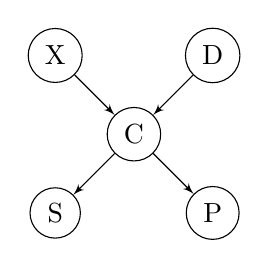
\begin{tikzpicture}
\tikzset{vertex/.style = {shape=circle,draw,minimum size=1.5em}}
\tikzset{edge/.style = {->,> = latex'}}
% vertices
\node[vertex] (x) at  (-1, 1)  {X};
\node[vertex] (d) at  (1, 1)   {D};
\node[vertex] (c) at  (0, 0)   {C};
\node[vertex] (s) at  (-1, -1) {S};
\node[vertex] (p) at  (1, -1)  {P};
%edges
\draw[edge] (x) to (c);
\draw[edge] (d) to (c);
\draw[edge] (c) to (s);
\draw[edge] (c) to (p);
\end{tikzpicture}
\end{figure}

			\textbf{Link from X - C:} A positive X-Ray implies that you are more likely to have cancer\\
			\textbf{Link from D - C:} If a patient has Dyspnoea then this condition increases the likelihood that they have cancer.\\
			\textbf{Link from C - S:} A patient who has cancer would be more likely to be a smoker\\
			\textbf{Link from C - P:} A patient who has cancer is more likely to have been exposed to pollution\\
			
\end{document}